%template1.tex
%The following LaTeX source file represents the simplest kind of slide presentation; no overlays, no included graphics. Substitute your favorite style for ``pascal''. To create the PDF file template1.pdf, (1) be sure to use the prosper class, then (2) execute the command latex template1.tex, and (3) the command dvipdf template1.dvi.

%%%%%%%%%%%%%%%%%%%%%%%%%%%%%%% template1.tex %%%%%%%%%%%%%%%%%%%%%%%%%%%%%%%%%%%
\documentclass[a4paper,blends,pdf,colorBG,slideColor]{prosper}
% definitions for slides for CSC544
% Lutz Hamel, (c) 2007

\hypersetup{pdfpagemode=FullScreen}

\usepackage{times}
\usepackage{latexsym}
\usepackage{alltt}
\usepackage{booktabs}
\usepackage{amsmath}
\usepackage{amsopn}
\usepackage{amsfonts}
\usepackage{amssymb}
%\usepackage[usenames]{color}

\def\sign{\qopname\relax{no}{sign}}
\def\argmax{\qopname\relax{no}{argmax}}
\def\argmin{\qopname\relax{no}{argmin}}

\newcommand{\grad}{\ensuremath{\nabla}} 
\newcommand{\loss}{\ensuremath{{\cal L}}}
\newcommand{\err}{\mbox{err}}
\newcommand{\mse}{\mbox{mse}}
\newcommand{\acc}{\mbox{acc}}
\newcommand{\Integer}{\ensuremath{\mathbb{N}}}
\newcommand{\size}[1]{{|{#1}|}}
\newcommand{\Rnspace}[1]{\ensuremath{\mathbb{R}^{#1}}}
\newcommand{\Real}{\ensuremath{\mathbb{R}}}
\newcommand{\mytt}[1]{{\small\tt{#1}}}
\newcommand{\textemph}[1]{{\em #1}}
\newcommand{\suchthat}{\mid}
\newcommand{\orbar}{\;|\;}
\newcommand{\bs}[1]{\begin{slide}{#1}\ptsize{8}}
\newcommand{\es}{\end{slide}}
\newcommand{\co}{\,\colon\;}
\newcommand{\pair}[2]{\ensuremath{( {#1}, {#2} )}}
\newcommand{\model}[1]{\hat{#1}}
\newcommand{\ul}[1]{{\bf\em #1}}
\newcommand{\ol}{\overline}
\newcommand{\definition}[1]{{\bf Definition: }{\em #1}}
\newcommand{\example}[1]{{\bf Example: }{#1}}
\newcommand{\abs}[1]{|{#1}|}
\newcommand{\mytab}{\makebox[.1in]{}}

\newcommand{\fdef}[1]{
\begin{center}
\fbox{
\begin{minipage}{3.5in}
{\bf Definition:}
{#1}
\end{minipage}
}
\end{center}
}

\newcommand{\fframe}[1]{
\begin{center}
\fbox{
\begin{minipage}{3.5in}
{#1}
\end{minipage}
}
\end{center}
}

\newcommand{\nframe}[1]{
\begin{center}
\begin{minipage}{3.5in}
{#1}
\end{minipage}
\end{center}
}

\newenvironment{Rcode}
	{
		\scriptsize
		\begin{quote}
		\begin{alltt}
	}
	{
		\end{alltt}
		\end{quote}
	}




\begin{document}
\bs{Perceptron Learning}
In 1953 Frank Rosenblatt invented another way of calculating a decision surface
for a binary classification problem - {\bf\em The Perceptron}.

The perceptron is the precursor of our modern artificial neural networks.
\begin{center}
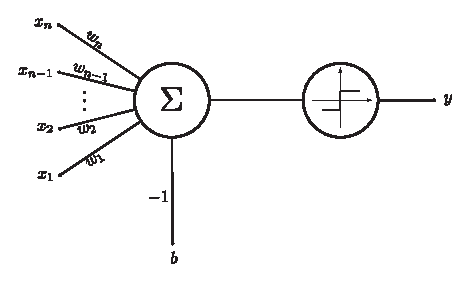
\includegraphics[height=30mm]{figures/fig05-01.eps}
\end{center}
It is not difficult to see that a perceptron computes the following decision function
\[
\model{f}(\ol{x})= y = \sign\left(\left[\sum_{k=1}^n w_k x_k\right] + (-1) b\right) = \sign\left(\ol{w}\bullet\ol{x} - b\right).
\]
where $\ol{w} = (w_1, w_2, \ldots, w_n)$ and $\ol{x} = (x_1, x_2,\ldots,x_n)$.
The free parameters of the perceptron are $\ol{w}$ and $b$ and they need to be
estimated using some training set $D$.

\es

\bs{Perceptron Learning}
Here $\ol{w}$ and $b$ are called the {\bf\em free parameters} of the perceptron.

Estimating the free parameters using the training set $D$ is called (perceptron) {\bf\em learning}.  Here $D$ has the usual structure $\pair{\ol{x}}{y} \in D$ with
$\ol{x} \in \Rnspace{n}$ and $y \in \{+1,-1\}$.

The {\bf\em learning algorithm} is as follows:

\begin{center}
\fbox{
\begin{minipage}{1.5in}
{\small
Initialize $\ol{w}$ and $b$ to random values.\\
Do\\
\mytab For each $\pair{\ol{x}}{y} \in D$ do\\
\mytab\mytab if $\model{f}(\ol{x}) \ne y$ then\\
\mytab\mytab\mytab Update $\ol{w}$ and $b$\\
\mytab\mytab end if\\
\mytab end for\\
Until $D$ is perfectly classified\\
Return $\ol{w}$ and $b$
}
\end{minipage}
}
\end{center}
\es

\bs{Perceptron Learning}

{\bf Observations:}

\begin{itemize}

\item The inherent assumption is that $D$ is linearly separable, that is,
a hyperplane can be found that perfectly separates the two classes.
The learning algorithm will not converge if the dataset is not linearly separable.

\item The computation stops as soon  as no more mistakes are made on 
classifying the training set $D$.  This might lead to suboptimal decision surfaces.
Compare this to our previous learning algorithm where we made sure that
the  decision surface is placed half way between the to means of the classes, respectively.

\end{itemize}
\es

\bs{Perceptron Learning}
\begin{center}
\fbox{
\begin{minipage}{3in}
{\small
{\bf let} $D = \{(\ol{x}_1,y_1), (\ol{x}_2,y_2),\dots,(\ol{x}_l,y_l)\} \subset \Rnspace{n} \times \{+1, -1\}$\\{\bf let} $0 < \eta <1$\\
$\ol{w} \leftarrow \ol{0}$\\
$b \leftarrow 0$\\
$r \leftarrow \max \{ \abs{\ol{x}} \mid (\ol{x},y)\in D\}$\\
{\bf repeat}\\
\mytab {\bf for} $i = 1$ {\bf to} $l$\\
\mytab\mytab {\bf  if} $\sign(\ol{w}\bullet\ol{x}_i - b) \neq y_i$ {\bf then}\\
\mytab\mytab\mytab $\ol{w} \leftarrow \ol{w} + \eta y_i \ol{x}_i$\\
\mytab\mytab\mytab $b \leftarrow b - \eta y_i r^2$\\
\mytab\mytab {\bf end if}\\
\mytab {\bf end for}\\
{\bf until} $\sign(\ol{w}\bullet\ol{x}_j - b) = y_j$ {\rm with} $j = 1,\ldots,l$\\
{\bf return} $(\ol{w}, b)$
}
\end{minipage}
}
\end{center}
\es

\bs{Perceptron Learning}
The effect of the perceptron update rule that changes the normal vector 
of a decision surface $\ol{w} \leftarrow \ol{w} + \eta \ol{x}_i$ using
$(\ol{x}_1,+1)\in D$,

\vspace{.2in}
\begin{center}
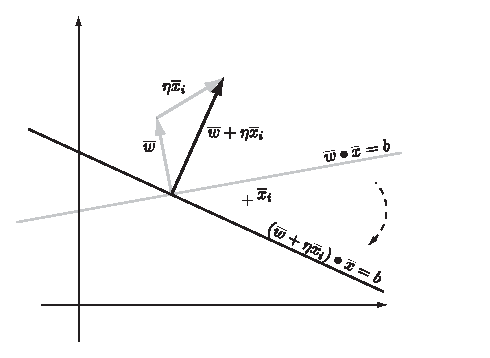
\includegraphics[height=45mm]{figures/fig05-02.eps}
\end{center}

\es

\bs{Perceptron Learning}
The effect of the perceptron update rule that changes the offset term 
of a decision surface $b \leftarrow b - \eta  r^2$ using
$(\ol{x}_1,+1)\in D$,

\vspace{.2in}
\begin{center}
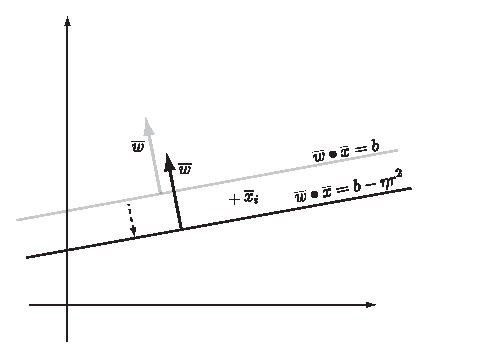
\includegraphics[height=45mm]{figures/fig05-03.eps}
\end{center}

\es

\bs{Perceptron Learning}
\begin{center}
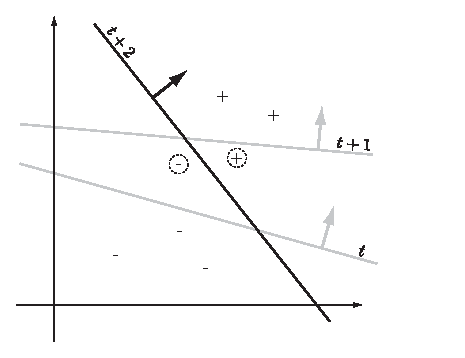
\includegraphics[height=50mm]{figures/fig05-04.eps}
\end{center}
{\tiny <demo>}
\es

\bs{Perceptron Learning}
{\bf Observations:} 
\begin{itemize}
\item The perceptron learning algorithm is a heuristic search in $\ol{w}$-$b$-space.
\item The search terminates as soon as {\em some} decision surface has been found.
\item There is no guarantee of ``optimality''.\footnote{In absence of any other information we consider
the optimal decision surface to lie right in the middle between the two classes.}
\item However, notice that points far away from the boundary between the classes have very little impact
on the solution.
\end{itemize}

\vspace{.1in}
$\Rightarrow$ This means we are kind of stuck, the ``simple learning algorithm" constructed an optimal decision
surface but was sensitive to outliers; the perceptron is not sensitive to outliers but its learning algorithm provides no
guarantees with respect to the quality of the decision surface.
\es

\end{document}
%%%%%%%%%%%%%%%%%%%%%%%%%%% end of template1.tex %%%%%%%%%%%%%%%%%%%%%%%%%%%%%%%%

